%%%%%%%%%%%%%%%%%%%%%%%%%%%%%%%%%%%%%%%%%
% Beamer Presentation
% LaTeX Template
% Version 1.0 (10/11/12)
%
% This template has been downloaded from:
% http://www.LaTeXTemplates.com
%
% License:
% CC BY-NC-SA 3.0 (http://creativecommons.org/licenses/by-nc-sa/3.0/)
%
%%%%%%%%%%%%%%%%%%%%%%%%%%%%%%%%%%%%%%%%%

%----------------------------------------------------------------------------------------
%	PACKAGES AND THEMES
%----------------------------------------------------------------------------------------

\documentclass{beamer}

\mode<presentation> {

% The Beamer class comes with a number of default slide themes
% which change the colors and layouts of slides. Below this is a list
% of all the themes, uncomment each in turn to see what they look like.

%\usetheme{default}
%\usetheme{AnnArbor}
%\usetheme{Antibes}
%\usetheme{Bergen}
%\usetheme{Berkeley}
%\usetheme{Berlin}
%\usetheme{Boadilla}
\usetheme{CambridgeUS}
%\usetheme{Copenhagen}
%\usetheme{Darmstadt}
%\usetheme{Dresden}
%\usetheme{Frankfurt}
%\usetheme{Goettingen}
%\usetheme{Hannover}
%\usetheme{Ilmenau}
%\usetheme{JuanLesPins}
%\usetheme{Luebeck}
%\usetheme{Madrid}
%\usetheme{Malmoe}
%\usetheme{Marburg}
%\usetheme{Montpellier}
%\usetheme{PaloAlto}
%\usetheme{Pittsburgh}
%\usetheme{Rochester}
%\usetheme{Singapore}
%\usetheme{Szeged}
%\usetheme{Warsaw}

% As well as themes, the Beamer class has a number of color themes
% for any slide theme. Uncomment each of these in turn to see how it
% changes the colors of your current slide theme.

%\usecolortheme{albatross}
%\usecolortheme{beaver}
%\usecolortheme{beetle}
%\usecolortheme{crane}
%\usecolortheme{dolphin}
%\usecolortheme{dove}
%\usecolortheme{fly}
%\usecolortheme{lily}
%\usecolortheme{orchid}
%\usecolortheme{rose}
%\usecolortheme{seagull}
%\usecolortheme{seahorse}
%\usecolortheme{whale}
%\usecolortheme{wolverine}

%\setbeamertemplate{footline} % To remove the footer line in all slides uncomment this line
%\setbeamertemplate{footline}[page number] % To replace the footer line in all slides with a simple slide count uncomment this line

%\setbeamertemplate{navigation symbols}{} % To remove the navigation symbols from the bottom of all slides uncomment this line
}

\usepackage{graphicx} % Allows including images
\usepackage{booktabs} % Allows the use of \toprule, \midrule and \bottomrule in tables
\usepackage{multirow}
\usepackage{color}

\newcommand{\blue}[1]{\textcolor{blue}{#1}}
\newcommand{\red}[1]{\textcolor{red}{#1}}
\newcommand{\green}[1]{\textcolor{green}{#1}}
\newcommand{\yellow}[1]{\textcolor{yellow}{#1}}
\newcommand{\orange}[1]{\textcolor{orange}{#1}}
\newcommand{\cyan}[1]{\textcolor{cyan}{#1}}
\newcommand{\magenta}[1]{\textcolor{magenta}{#1}}
%----------------------------------------------------------------------------------------
%	TITLE PAGE
%----------------------------------------------------------------------------------------

\title[Circuit(ENGG 1203)]{Tutorial on Circuit (Part 2) \newline Introduction to Electrical and Electronic Engineering} % The short title appears at the bottom of every slide, the full title is only on the title page

\author{Nan Meng} % Your name
\institute[Imaging Systems Laboratory] % Your institution as it will appear on the bottom of every slide, may be shorthand to save space
{
	University of Hong Kong \\ % Your institution for the title page
	\medskip
	\textit{u3003637@connect.hku.hk} % Your email address
}
\date{\today} % Date, can be changed to a custom date

\begin{document}

\begin{frame}
	\titlepage % Print the title page as the first slide
\end{frame}

\begin{frame}
\frametitle{Overview} % Table of contents slide, comment this block out to remove it

\begin{itemize} \itemsep1pt \parskip0pt \parsep0pt
  \item[$\ast$] {\bf Learning Objectives:}\newline Analyze circuits with ideal operational amplifiers
  \item[$\ast$] {\bf Basics}
  \begin{itemize} \itemsep1pt \parskip0pt \parsep0pt
    \item[$\bullet$] Symbols \& Rules
    \item[$\bullet$] Operational Amplifiers
    \begin{itemize} \itemsep1pt \parskip0pt \parsep0pt
      \item[$\bullet$] \red{The Ideal op-amp Model}
      \item[$\bullet$] \red{Ideal op-amp in a negative feedback configuration}
    \end{itemize}
  \end{itemize}
  \item[$\ast$] {\bf Questions \& Summary}
\end{itemize}
\end{frame}

%----------------------------------------------------------------------------------------
%	PRESENTATION SLIDES
%----------------------------------------------------------------------------------------

%------------------------------------------------

%------------------------------------------------

\begin{frame}
\frametitle{Symbols \& Rules(Recap)}

\begin{itemize}
  \item {\bf \blue{Operational Amplifiers}}
\end{itemize}
\begin{figure}[H]
  \centering
  \includegraphics[width=0.4\textwidth]{./image/circuit2/circuit_append}
  \caption{{\bf Equivalent circuit model of op-amp device}}
\end{figure}
\centerline{In the absence of any load at the output, the output voltage is }
\centerline{$V_o = AV_i = A(V_p - V_n)$}

\end{frame}


%------------------------------------------------
%------------------------------------------------

\begin{frame}
\frametitle{Operational Amplifiers(Recap)}

\begin{itemize}
  \item {\bf \blue{Operational Amplifiers}}
\end{itemize}

\centerline{In the absence of any load at the output, the output voltage is }
\centerline{$V_o = AV_i = A(V_p - V_n)$}

\begin{block}{}
Which indicates that the output voltage $V_o$ is a function of the difference between the input voltages $V_p$ and $V_n$. For this reason op-amps are {\bf difference amplifiers}. 
\end{block}

\end{frame}


%------------------------------------------------
%------------------------------------------------

\begin{frame}
\frametitle{Operational Amplifiers(Recap)}

\begin{itemize}
  \item {\bf \blue{The Ideal Op-amp Model}}
\end{itemize}
\begin{figure}[H]
  \centering
  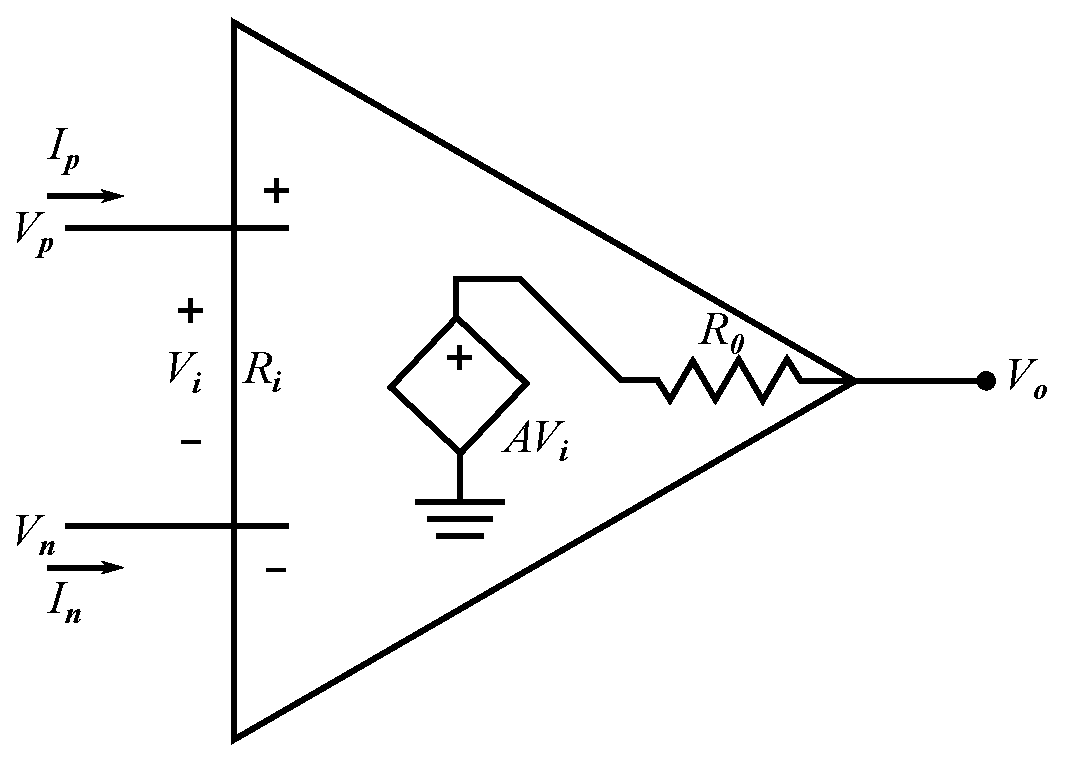
\includegraphics[width=0.4\textwidth]{./image/circuit2/circuit_append1}
  \caption{{\bf Ideal op-amp model}}
\end{figure}

\end{frame}


%------------------------------------------------
\begin{frame}
\frametitle{Operational Amplifiers(Recap)}
An ideal op-amp is a device which acts as an ideal voltage
controlled voltage source. Referring to Figure in the previous slide, this implies that the device will have the
following characteristics:
\begin{itemize}
  \item[$\ast$] {\bf No current flows into the input terminals} of the device. This is equivalent to having an infinite input resistance \red{\bf $R_i = \infty$}. In practical terms this implies that the amplifier device will make no power demands on the input signal source.
  \item[$\ast$] {\bf Have a zero output resistance} \red{$(R_o=0)$}. This implies that the output voltage is independent of the load connected to the output.
\end{itemize}
\end{frame}
%------------------------------------------------
%------------------------------------------------

\begin{frame}
\frametitle{Operational Amplifiers(Recap)}

\begin{itemize}
  \item {\bf \blue{The Ideal Op-amp Model}}
\end{itemize}

\begin{columns}
\begin{column}{4cm}
\begin{figure}[H]
  \centering
  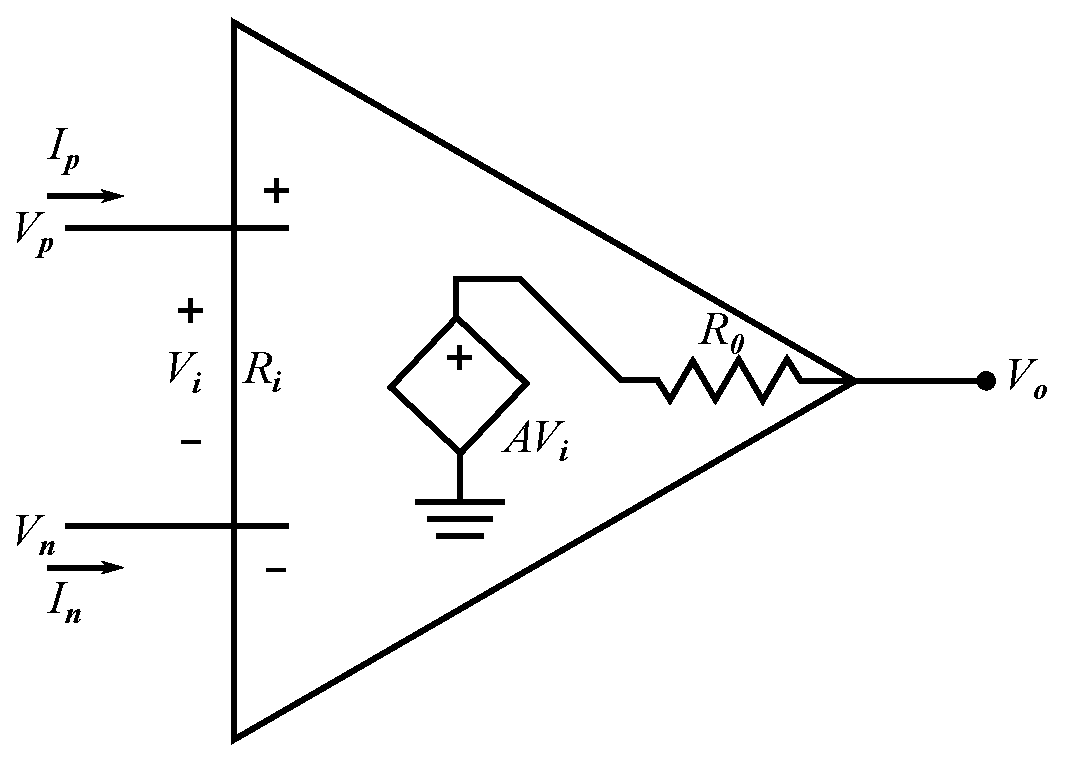
\includegraphics[width=1\textwidth]{./image/circuit2/circuit_append1}
  \caption{{\bf Ideal op-amp model}}
\end{figure}
\end{column}

\begin{column}{8cm}
\begin{itemize}
  \item[$\ast$] In summary, the ideal op-amp conditions are:
  \begin{itemize}
    \item[$\bullet$] $I_p = I_n = 0$ ~~\orange{\bf No current into the input}
    \item[] \hspace{20 mm}\orange{\bf terminals}
    \item[$\bullet$] $R_i \rightarrow \infty$ \hspace{7 mm}\orange{\bf Infinite input resistance}
    \item[$\bullet$] $R_o = 0$ \hspace{8 mm} \orange{\bf Zero output resistance}
    \item[$\bullet$] $A \rightarrow \infty$ \hspace{8 mm}\orange{\bf Infinite open loop gain}
  \end{itemize}
\end{itemize}
\end{column}
\end{columns}

\end{frame}


%------------------------------------------------
%------------------------------------------------
\begin{frame}
\frametitle{Operational Amplifiers(Recap)}

\begin{itemize}
  \item When an op-amp is arranged with a {\bf negative feedback} the ideal rules are: 
  \item[$\ast$] $I_p = I_n = 0$: input current constraint
  \item[$\ast$] $V_n = V_p$: \hspace{4 mm}input voltage constraint
\end{itemize}

\begin{figure}[H]
  \centering
  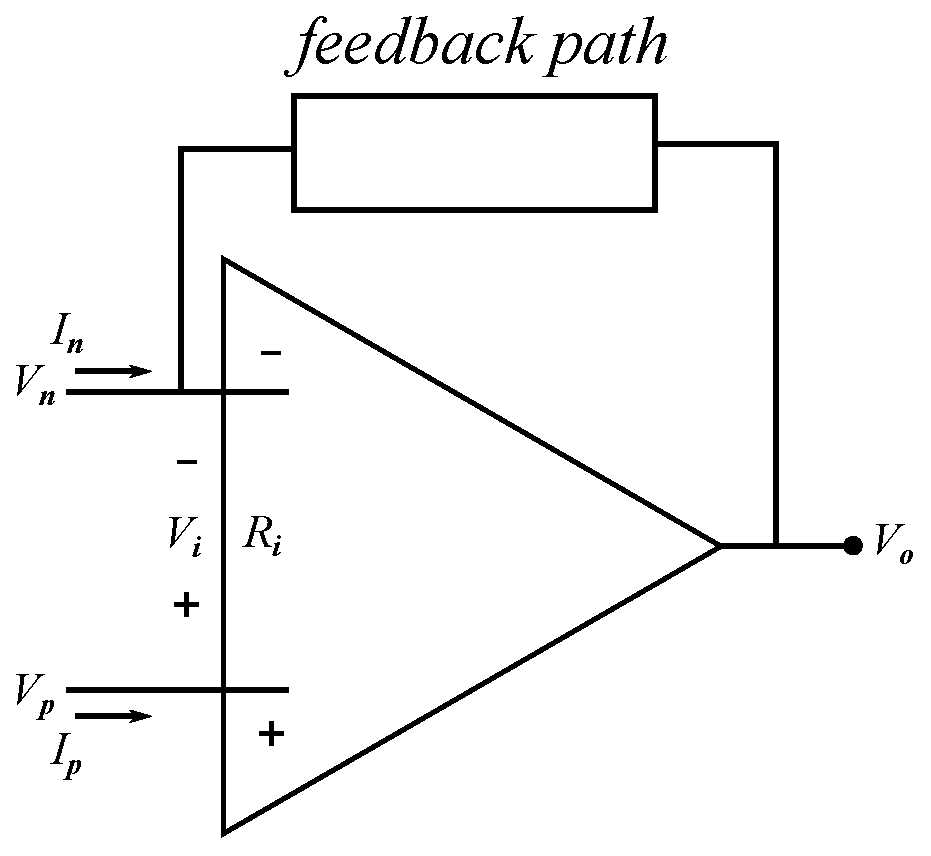
\includegraphics[width=0.36\textwidth]{./image/circuit2/circuit_append2}
  \caption{{\bf Basic negative feedback configuration. }}
\end{figure}
% \begin{block}{}
% These rules are related to the requirement/assumption for large open-loop gain $A \rightarrow \infty$, and they form the basis for op-amp circuit analysis.
% \end{block}

% \begin{block}{}
% The voltage $V_n$ tracks the voltage $V_p$ and the ``control'' of $V_n$ is accomplished via the feedback network.
% \end{block}

\end{frame}
%------------------------------------------------
%------------------------------------------------

\begin{frame}
\frametitle{Question 1}

\begin{itemize} \itemsep1pt \parskip0pt \parsep0pt
  \item[$\ast$] \blue{Determine $V_0$ in the following circuit. Assume that the op-amp is ideal.}
\end{itemize}



\begin{figure}[H]
  \centering
  \includegraphics[width=0.6\textwidth]{./image/circuit2/circuit1_0}
\end{figure}


\end{frame}

%------------------------------------------------
%------------------------------------------------

\begin{frame}
\frametitle{Solution(Q1)}

\begin{itemize} \itemsep1pt \parskip0pt \parsep0pt
  \item[$\ast$] Since $V_- = V_+$, $V - = 5V$. So there must be 1/12A flowing left through the two $6\Omega$ resistors($i_1 = \frac{1}{12}A$). There must be a corresponding 1/12A($i_2 = \frac{1}{12}A$) flowing to the left through the 12 ohm resistor. $V_0$ is then the sum of $V_- = 5V$ and the 1V across the $12\Omega$ resistor.
\end{itemize}



\begin{figure}[H]
  \centering
  \includegraphics[width=0.6\textwidth]{./image/circuit2/circuit1_1}
\end{figure}


\end{frame}

%------------------------------------------------
%------------------------------------------------

\begin{frame}
\frametitle{Question 2}
\begin{columns}
\begin{column}{6cm}
\begin{itemize} \itemsep1pt \parskip0pt \parsep0pt
  \item[$\ast$]Determine the current $I_x$ when $V_1 = 1V$ and $V_2 = 2V$.
  \item[$\ast$]Determine the voltage $V_A$ when $V_1 = 1V$ and $V_2 = 2V$.
  \item[$\ast$]Determine a general expression for $V_A$ in terms of $V_1$ and $V_2$.
\end{itemize}
\end{column}

\begin{column}{6cm}
\begin{figure}[H]
  \centering
  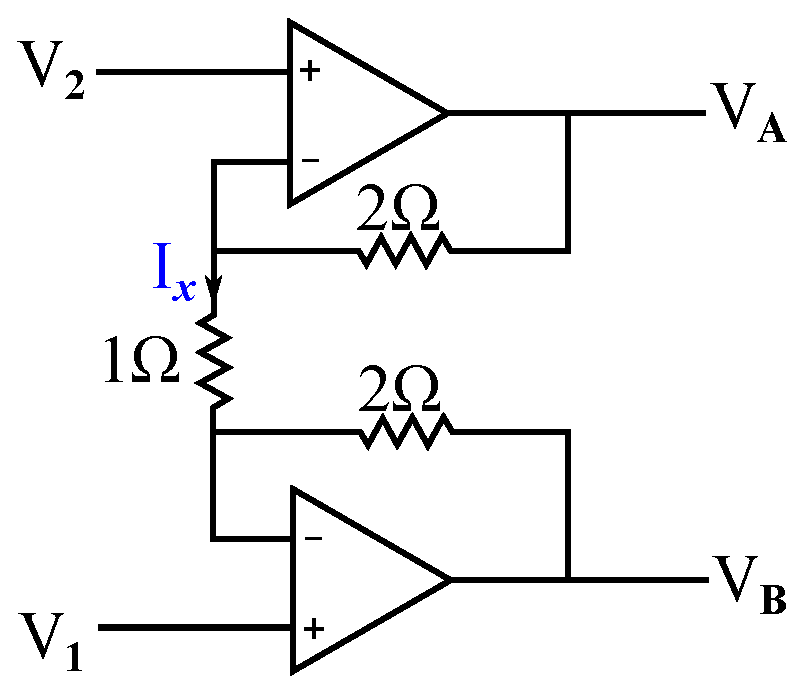
\includegraphics[width=0.8\textwidth]{./image/circuit2/circuit2_0}
\end{figure}
\end{column}
\end{columns}

\end{frame}

%------------------------------------------------
%------------------------------------------------

\begin{frame}
\frametitle{Solution(Q2)}
\begin{columns}
\begin{column}{7.5cm}
\begin{itemize} \itemsep1pt \parskip0pt \parsep0pt
  \item[$\ast$]\blue{Determine the current $I_x$ when \newline $V_1 = 1V$ and $V_2 = 2V$.}
  \item[$\ast$]\blue{Determine the voltage $V_A$ when \newline $V_1 = 1V$ and $V_2 = 2V$.}
  \item[$\ast$]\blue{Determine a general expression \newline for $V_A$ in terms of $V_1$ and $V_2$.}
\end{itemize}

\begin{itemize} \itemsep1pt \parskip0pt \parsep0pt
  \item[$\ast$] When $V_1 = 1V$ and $V_2 = 2V$, $I_x = 1A$
  \item[$\ast$] When $V_1 = 1V$ and $V_2 = 2V$, $V_A = 4V$
  \item[$\ast$] \red{A general expression for $V_A$:}
  \item[] \hspace{8 mm}\red{$V_A = V_2 + I_x \times 2$}
  \item[] \hspace{14 mm}\red{$=V_2 + \frac{V_2-V_1}{1} \times 2$}
  \item[] \hspace{14 mm}\red{$=V_2 + 2(V_2 - V_1)$}
  \item[] \hspace{14 mm}\red{$=-2V_1 + 3V_2$}
\end{itemize}


\end{column}

\begin{column}{5cm}
\begin{figure}[H]
  \centering
  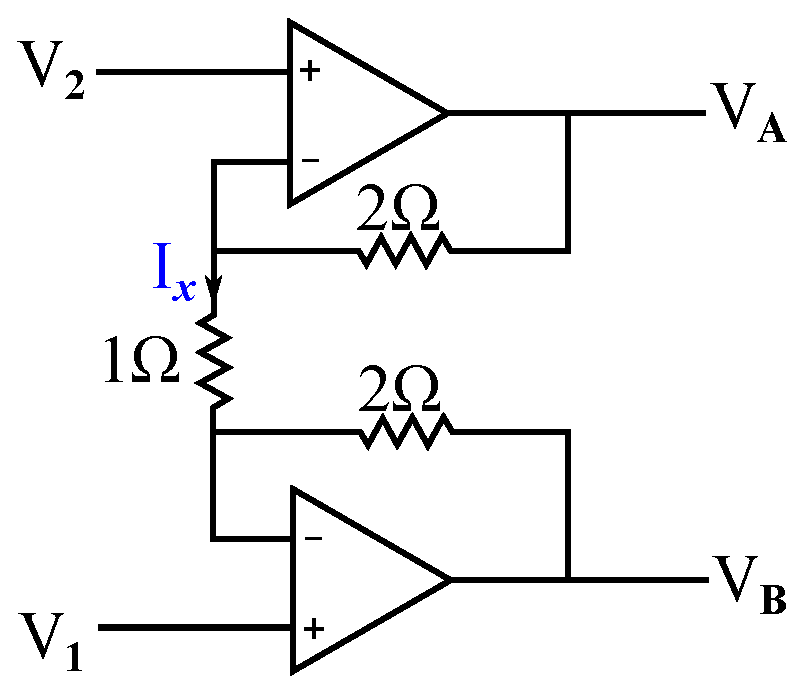
\includegraphics[width=1\textwidth]{./image/circuit2/circuit2_0}
\end{figure}
\end{column}
\end{columns}

\end{frame}

%------------------------------------------------
%------------------------------------------------

\begin{frame}
\frametitle{Question 3}

\begin{itemize} \itemsep1pt \parskip0pt \parsep0pt
  \item[$\ast$] Use a single op-amp and resistors to make a circuit that is equivalent to the following circuit.
\end{itemize}



\begin{figure}[H]
  \label{epi_circuit3}
  \centering
  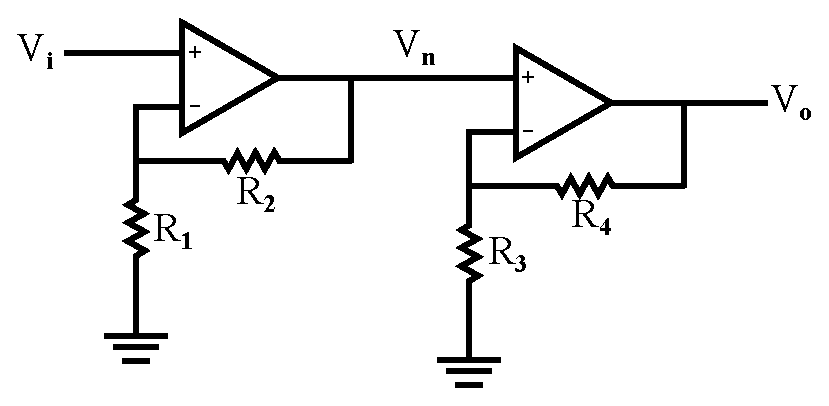
\includegraphics[width=0.6\textwidth]{./image/circuit2/circuit3_0}
\end{figure}


\end{frame}

%------------------------------------------------
%------------------------------------------------

\begin{frame}
\frametitle{Solution(Q3)}
\begin{columns}
\begin{column}{6cm}
\begin{itemize} \itemsep1pt \parskip0pt \parsep0pt
  \item[$\ast$] \blue{Use a single op-amp and resistors to make a circuit that is equivalent to the following circuit}.
\end{itemize}

\begin{itemize} \itemsep1pt \parskip0pt \parsep0pt
  \item[] $\frac{V_n}{V_i} = (1+\frac{R_2}{R_1})$
  \item[] $\frac{V_0}{V_i} = \frac{V_0}{V_n}\frac{V_n}{V_i} = (1+\frac{R_3}{R_4})(1+\frac{R_2}{R_1})$
  \item[] $1 + \frac{R_1R_4+R_2R_3+R_2R_4}{R_1R_3}$
\end{itemize}


\end{column}

\begin{column}{6cm}
\begin{figure}[H]
  \centering
  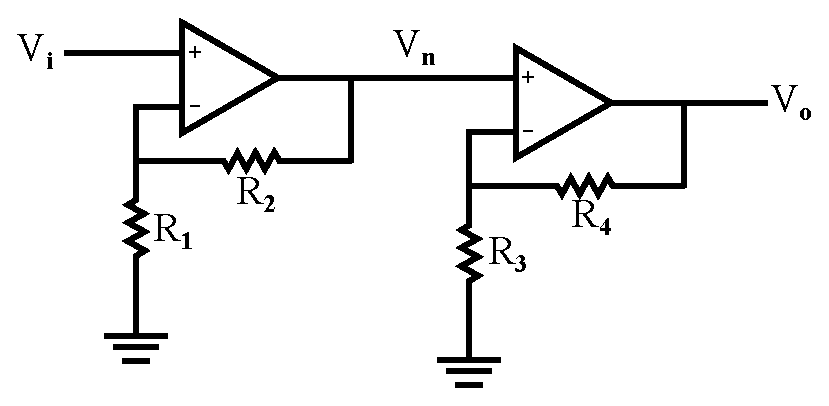
\includegraphics[width=1\textwidth]{./image/circuit2/circuit3_0}
\end{figure}

\begin{figure}[H]
  \centering
  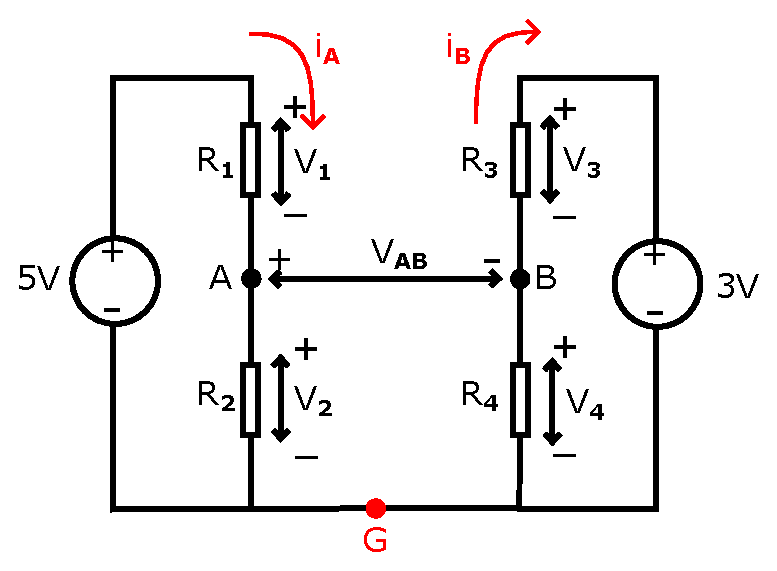
\includegraphics[width=0.8\textwidth]{./image/circuit2/circuit3_1}
\end{figure}

\end{column}
\end{columns}

\end{frame}

%------------------------------------------------
%------------------------------------------------

\begin{frame}
\frametitle{Question 4}

\begin{itemize} \itemsep1pt \parskip0pt \parsep0pt
  \item[$\ast$] \blue{Use the ideal op-amp model($V_+ = V_-$)to
determine an expression for the output current $I_0$
in terms of the input voltage $V_i$ and resistors $R_1$
and $R_2$.}
\end{itemize}



\begin{figure}[H]
  \centering
  \includegraphics[width=0.5\textwidth]{./image/circuit2/circuit4_0}
\end{figure}


\end{frame}

%------------------------------------------------
%------------------------------------------------

\begin{frame}
\frametitle{Solution(Q4)}

\begin{itemize} \itemsep1pt \parskip0pt \parsep0pt
  \item[$\ast$] \blue{Use the ideal op-amp model($V_+ = V_-$)to
determine an expression for the output current $I_0$
in terms of the input voltage $V_i$ and resistors $R_1$
and $R_2$.}
\end{itemize}


\begin{columns}
\begin{column}{6cm}
\begin{itemize} \itemsep1pt \parskip0pt \parsep0pt
  \item[] $V_x = (V_i + V_x)\frac{R_2}{R_1+R_2}$
  \item[$\Rightarrow$] $V_x = V_i\frac{R_2}{R_1}$ \newline
  \item[] $I_0 = \frac{V_x}{R_2} = \frac{1}{R_2}V_i\frac{R_2}{R_1} = \frac{V_i}{R_1}$
\end{itemize}
\end{column}


\begin{column}{6cm}
\begin{figure}[H]
  \centering
  \includegraphics[width=0.8\textwidth]{./image/circuit2/circuit4_0}
\end{figure}
\end{column}
\end{columns}

\end{frame}

%------------------------------------------------
%------------------------------------------------

\begin{frame}
\frametitle{Question 5}

\begin{itemize} \itemsep1pt \parskip0pt \parsep0pt
  \item[$\ast$] \blue{Determine R so that $V_0 = 2(V_1 - V_2)$.}
\end{itemize}


\begin{figure}[H]
  \centering
  \includegraphics[width=0.6\textwidth]{./image/circuit2/circuit5_01}
\end{figure}


\end{frame}

%------------------------------------------------
%------------------------------------------------

\begin{frame}
\frametitle{Solution(Q5)}
\begin{columns}
\begin{column}{7.6cm}
\begin{itemize} \itemsep1pt \parskip0pt \parsep0pt
  \item[$\ast$] \blue{\bf No current in $V_-$ or $V_+$ inputs:}
  \item[] $V_+=\frac{R}{1+R}V_1$
  \item[] $V_-=V_2 + \frac{1}{1+2}(V_0-V_2) = \frac{2}{3}V_2 + \frac{1}{3}V_0$
\end{itemize}
\end{column}



\begin{column}{4cm}
\begin{figure}[H]
  \centering
  \includegraphics[width=1\textwidth]{./image/circuit2/circuit5_01}
\end{figure}
\end{column}
\end{columns}

\begin{itemize} \itemsep1pt \parskip0pt \parsep0pt
  \item[$\ast$] \blue{\bf Ideal op-amp:}
  \item[] $V_+ = V_- \Rightarrow \frac{R}{1+R}V_1 = \frac{2}{3}V_2 + \frac{1}{3}V_0$
  \item[] $V_0 = \frac{3R}{1+R}V_1-2V_2$ ~~$\rightarrow$ ~~$\frac{3R}{1+R} = 2$ ~~$\rightarrow$ ~~$R = 2\Omega$
\end{itemize}

\end{frame}

%------------------------------------------------
%------------------------------------------------

\begin{frame}
\frametitle{Question 6}

\begin{itemize} \itemsep1pt \parskip0pt \parsep0pt
  \item[$\ast$] A proportional controller that regulates the
current through a motor by setting the motor
voltage \red{$V_C$} to \red{$V_C = K(I_d - I_0)$}
\end{itemize}


\begin{columns}

\begin{column}{4cm}
\begin{itemize} \itemsep1pt \parskip0pt \parsep0pt
  \item[$\ast$] $K$ is the gain(ohms)
  \item[$\ast$] $I_d$ is the desired motor current
  \item[$\ast$] $I_0$ is the actual current through the motor.
\end{itemize}
\end{column}


\begin{column}{8cm}
\begin{figure}[H]
  \centering
  \includegraphics[width=1\textwidth]{./image/circuit2/circuit6_0}
\end{figure}
\end{column}

\end{columns}

\end{frame}

%------------------------------------------------
%------------------------------------------------

\begin{frame}
\frametitle{Question 6}

\begin{itemize} \itemsep1pt \parskip0pt \parsep0pt
  \item[$\ast$] A proportional controller that regulates the
current through a motor by setting the motor
voltage \red{$V_C$} to \red{$V_C = K(I_d - I_0)$}
\end{itemize}


\begin{columns}

\begin{column}{4cm}
\begin{itemize} \itemsep1pt \parskip0pt \parsep0pt
  \item[$\ast$] \blue{Consider the circuit inside the dotted rectangle. Determine $V_1$ as a function of $I_o$}
  \item[$\ast$] \blue{Determine the gain K and desired motor current $I_d$}
\end{itemize}
\end{column}


\begin{column}{8cm}
\begin{figure}[H]
  \centering
  \includegraphics[width=1\textwidth]{./image/circuit2/circuit6_1}
\end{figure}
\end{column}

\end{columns}

\end{frame}

%------------------------------------------------
%------------------------------------------------

\begin{frame}
\frametitle{Solution(Q6)}

\begin{columns}

\begin{column}{6cm}
\begin{itemize} \itemsep1pt \parskip0pt \parsep0pt
  \item[$\ast$] Consider the circuit inside the dotted rectangle. Determine $V_1$ as a function of $I_0$.
  \item[$\ast$] $V_+ = 1/2 x I_0 = V_-$
  \item[] $V_- = 100/(100+9900) \times V_1$
  \item[$\Rightarrow$] \blue{$V_1 = 1/2 x I_0 \times 100$}
\end{itemize}
\end{column}


\begin{column}{7.5cm}
\begin{figure}[H]
  \centering
  \includegraphics[width=0.8\textwidth]{./image/circuit2/circuit6_1}
\end{figure}
\end{column}

\end{columns}

\begin{itemize} \itemsep1pt \parskip0pt \parsep0pt
  \item[$\ast$] Determine the gain $K$ and desired motor current $I_d$.
  \item[$\ast$] KCL at $V_-$ input to right op-amp:
  \item[] \hspace{6 mm}\red{$\frac{V_c-2.5}{1000}$} $= \frac{2.5-V_1}{1000} \Rightarrow V_c = 50(0.1-I_0)$
\end{itemize}
\end{frame}

%------------------------------------------------
%------------------------------------------------

\begin{frame}
\frametitle{Question 7}
\begin{itemize} \itemsep1pt \parskip0pt \parsep0pt
  \item[$\ast$]The following figure shows a motor controller. A \orange{\bf human} can turn the \orange{\bf left potentiometer} (the input pot). Then the \red{\bf motor} will turn the \red{\bf right potentiometer} (the output pot) so that the {\bf shaft angle of the output pot tracks that of the input pot.}
\end{itemize}



\begin{figure}[H]
  \centering
  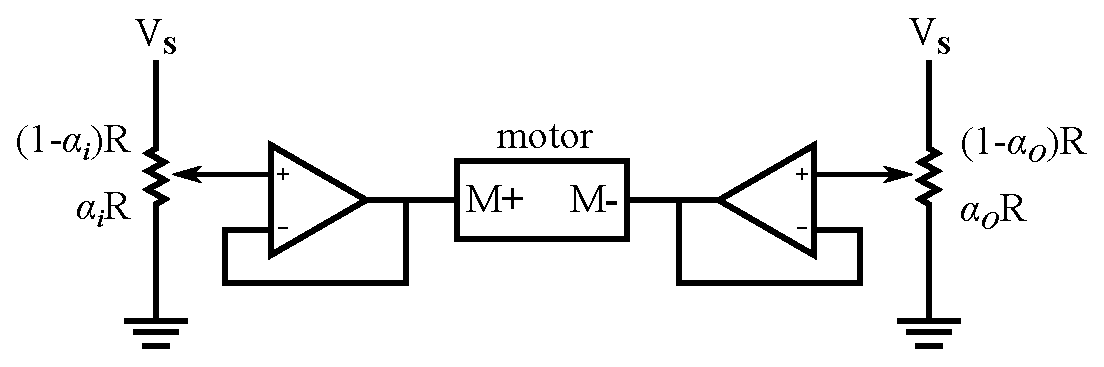
\includegraphics[width=0.8\textwidth]{./image/circuit2/circuit7_0}
\end{figure}



\end{frame}

%------------------------------------------------
%------------------------------------------------

\begin{frame}
\frametitle{Question 7}
\begin{itemize} \itemsep1pt \parskip0pt \parsep0pt
  \item[$\ast$] Pot resistances depends on shaft angle
  \begin{itemize} \itemsep1pt \parskip0pt \parsep0pt
  \item[$\bullet$] Lower part of the pot is $\alpha R$
  \item[$\bullet$] Upper part is $(1 - \alpha)R$, where $R = 1000\Omega$
  \item[$\bullet$] $\alpha$ is from $0$ (most counterclockwise position) to $1$ (most clockwise position)
  \end{itemize}
\end{itemize}

\begin{itemize} \itemsep1pt \parskip0pt \parsep0pt
  \item[$\ast$] If $\alpha_i > \alpha_o$ , then the voltage to the motor ($V_{M+} - V_{M-}$) is positive, and the motor turns clockwise (so as to increase $\alpha_o$ ) -- i.e., {\bf positive motor voltage $\rightarrow$ clockwise rotation.}
\end{itemize}

\begin{figure}[H]
  \centering
  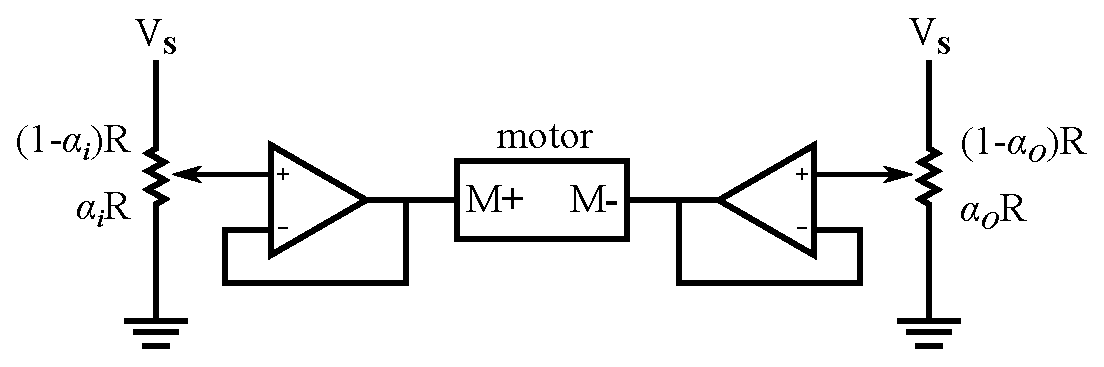
\includegraphics[width=0.8\textwidth]{./image/circuit2/circuit7_0}
\end{figure}



\end{frame}

%------------------------------------------------
%------------------------------------------------

\begin{frame}
\frametitle{Question 7(a)}
\begin{itemize} \itemsep1pt \parskip0pt \parsep0pt
  \item[$\ast$] Determine an expression for $V_{M+}$ in terms of $\alpha_i$, $R$, and $V_s$.
\end{itemize}


\begin{figure}[H]
  \centering
  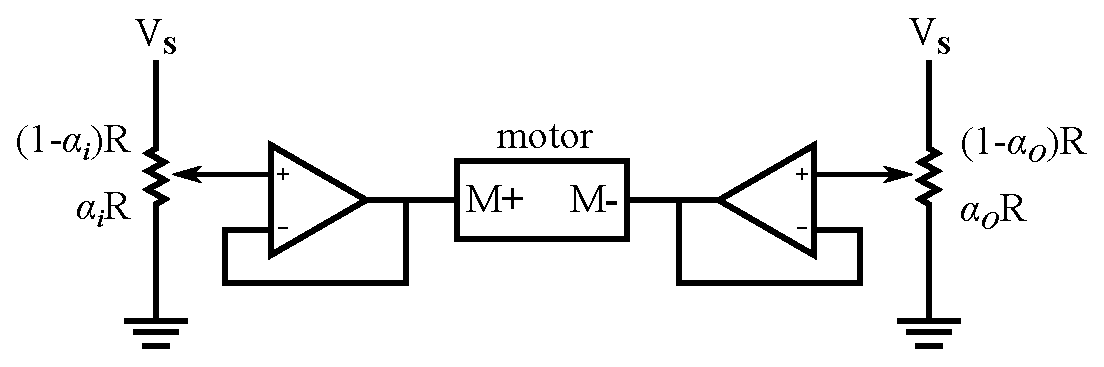
\includegraphics[width=0.8\textwidth]{./image/circuit2/circuit7_0}
\end{figure}

\end{frame}

%------------------------------------------------
%------------------------------------------------

\begin{frame}
\frametitle{Solution(Q7(a))}
\begin{itemize} \itemsep2pt \parskip0pt \parsep0pt
  \item[$\ast$] \blue{Determine an expression for $V_{M+}$ in terms of $\alpha_{i}$, $R$, and $V_S$.}
  \item[$\ast$] The output of the voltage divider is
  \item[] \hspace{3 cm} \red{$V_+ = \frac{\alpha_iR}{\alpha_iR + (1-\alpha_i)R}V_S = \alpha_iV_S$}
  \item[$\ast$] The op-amp provides a gain of 1, so $V_{M+} = V_+$.
\end{itemize}


\begin{figure}[H]
  \centering
  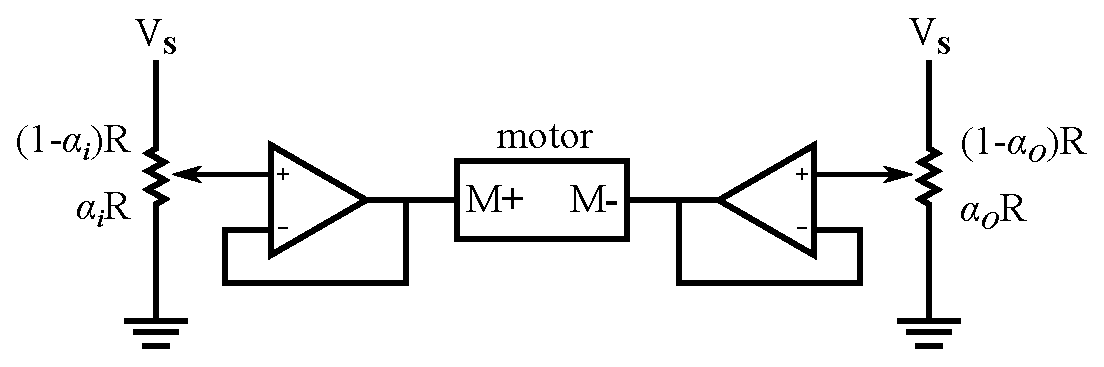
\includegraphics[width=0.8\textwidth]{./image/circuit2/circuit7_0}
\end{figure}

\end{frame}

%------------------------------------------------
%------------------------------------------------

\begin{frame}
\frametitle{Question 7(b)}
\begin{columns}
\begin{column}{6 cm}
\begin{itemize} \itemsep1pt \parskip0pt \parsep0pt
  \item[$\ast$] The following circuit produces a voltage $V_o$ that depends on the position of the input pot. Determine an expression for the voltage $V_o$ in terms of $\alpha_i$, $R$, $R_1$, $R_2$, and $V_s$.
\end{itemize}
\vspace{40 mm}
\end{column}
\begin{column}{6 cm}
\begin{figure}[H]
  \centering
  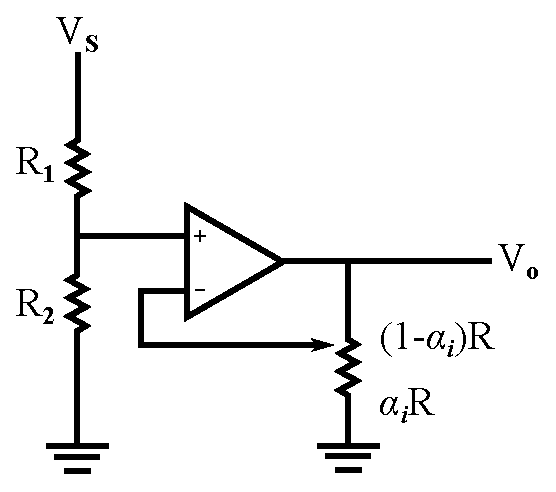
\includegraphics[width=0.8\textwidth]{./image/circuit2/circuit7_1}
\end{figure}
\end{column}
\end{columns}
\end{frame}

%------------------------------------------------
%------------------------------------------------

\begin{frame}
\frametitle{Solution(Q7(b))}
\begin{columns}

\begin{column}{6cm}
\begin{itemize} \itemsep1pt \parskip0pt \parsep0pt
  \item[$\ast$] \blue{The following circuit produces a voltage $V_o$ that depends on the position of the input pot. {\bf Determine an expression for the voltage $V_o$ in terms of $\alpha_i$, $R$, $R_1$, $R_2$ and$V_s$.}}
\end{itemize}
\end{column}


\begin{column}{6cm}
\begin{figure}[H]
  \centering
  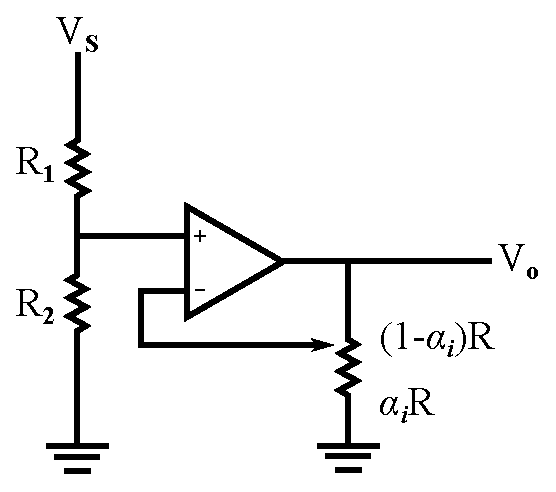
\includegraphics[width=0.8\textwidth,height=0.45\textheight]{./image/circuit2/circuit7_1}
\end{figure}
\end{column}

\end{columns}


\begin{itemize} \itemsep1pt \parskip0pt \parsep0pt
  \item[$\ast$] The positive input to the op-amp is connected to a voltage divider with equal resistors so
  \item[] \red{$V_+ = \frac{R_2}{R_1 + R_2}V_s$}
  \item[$\ast$] The input pot is on the output of the op-amp, so
  \item[] \red{$V_- = \frac{\alpha_iR}{\alpha_iR + (1-\alpha_i)R}V_o = \alpha_iV_o$}
  \item[$\ast$] In an ideal op-amp, $V_+ = V_-$ so \red{$V_o = \frac{R_2V_s}{(R_1 + R_2)\alpha_i}$}
\end{itemize}


\end{frame}

%------------------------------------------------
%------------------------------------------------

\begin{frame}
\frametitle{Question 7(c)}
\begin{columns}
\begin{column}{6 cm}
\begin{itemize} \itemsep1pt \parskip0pt \parsep0pt
  \item[$\ast$] The following circuit produces a voltage $V_o$ that depends on the positions of both pots. {\bf Determine an expression for $V_o$ in terms of $\alpha_i$, $\alpha_o$, $R$, and $V_s$}
\end{itemize}
\vspace{6 cm}
\end{column}
\begin{column}{6 cm}
\begin{figure}[H]
  \centering
  \includegraphics[width=0.8\textwidth]{./image/circuit2/circuit7_2}
\end{figure}
\end{column}
\end{columns}
\end{frame}

%------------------------------------------------
%------------------------------------------------

\begin{frame}
\frametitle{Solution(Q7(c))}

\begin{itemize} \itemsep1pt \parskip0pt \parsep0pt
  \item[$\ast$] \blue{The following circuit produces a voltage $V_0$ that depends on the position of the input pot. Determine an expression for the voltage $V_o$ in terms of $\alpha_i$, $\alpha_o$, $R$ and $V_s$.}
  \item[$\ast$] The positive input to the op-amp is connected to pot 1 so that
  \item[] \red{$V_+ = \frac{\alpha_iR}{\alpha_iR+(1-\alpha_i)R+R}V_s = \frac{\alpha_iV_s}{2}$}
\end{itemize}


\begin{columns}

\begin{column}{6cm}
\begin{itemize} \itemsep1pt \parskip0pt \parsep0pt
  \item[$\ast$] The output pot is on the output of the op-amp, so
  \item[] \red{$V_- = \frac{\alpha_oR}{\alpha_oR+(1-\alpha_o)R}V_o = \alpha_oV_o$}
  \item[$\ast$] In an ideal op-amp, $V_+ = V_-$ so \red{$V_o = \frac{\alpha_i}{\alpha_o}\frac{V_s}{2}$}
\end{itemize}
\end{column}


\begin{column}{6cm}
\begin{figure}[H]
  \centering
  \includegraphics[width=0.7\textwidth]{./image/circuit2/circuit7_2}
\end{figure}
\end{column}

\end{columns}



\end{frame}

%------------------------------------------------
%------------------------------------------------

\begin{frame}
\frametitle{Question 7(d)}
\begin{itemize} \itemsep2pt \parskip0pt \parsep0pt
  \item[$\ast$] Assume that we are provided with a circuit whose output is $\alpha_i/\alpha_o$ volts. We want to {\bf design a motor controller} of the following form so that the motor shaft angle (which is proportional to $\alpha_o$) will track the input pot angle (which is proportional to $\alpha_i$).
  \item[$\ast$] Assume that $R_1 = R_3 = R_4 = 1000\Omega$ and $V_C = 0$. Is it possible to choose $R_2$ \underline{so that $\alpha_o$ tracks $\alpha_i$}? If {\bf yes}, enter an acceptable value for $R_2$.
\end{itemize}


\begin{figure}[H]
  \centering
  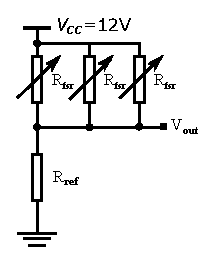
\includegraphics[width=0.5\textwidth]{./image/circuit2/circuit7_3}
\end{figure}

\end{frame}

%------------------------------------------------
%------------------------------------------------

\begin{frame}
\frametitle{Solution(Q7(d))}
\begin{itemize} \itemsep2pt \parskip0pt \parsep0pt
  \item[$\ast$] \blue{Assume that $R_1 = R_3 = R_4 = 1000\Omega$ and $V_C = 0$}
  \item[$\ast$] If $R_3 = R_4$ then the right motor input is 5V. If \red{$\alpha_i = \alpha_o$}then the gain of the {\bf left} op-amp circuit must be \red{\bf 5} so that the motor voltage is 0. The gain is $R_1 + R_2/R_1$, so $R_2$ must be $4000\Omega$.
\end{itemize}


\begin{figure}[H]
  \centering
  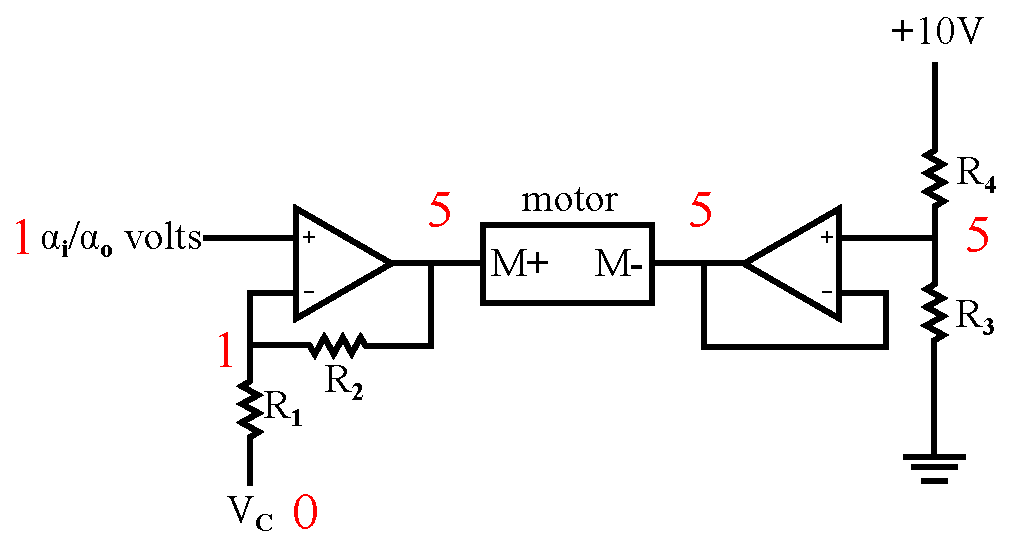
\includegraphics[width=0.6\textwidth]{./image/circuit2/circuit7_4}
\end{figure}

\end{frame}

%------------------------------------------------
%------------------------------------------------

\begin{frame}
\frametitle{Solution(Q7(d))}
\begin{itemize} \itemsep2pt \parskip0pt \parsep0pt
  \item[$\ast$] \blue{Assume that $R_1 = R_3 = R_4 = 1000\Omega$ and} \red{$V_C = 5V$}
  \item[$\ast$] If $R_3 = R_4$ then the right motor input is 5V. If $\alpha_i = \alpha_o$ then $V_+ = V_- = 1$ for the right op-amp. We need the left motor input to be 5V. But if the left motor input is 5V and $V_C = 5V$ then $V_-$ must also be 5V, which leads to a contradiction.
\end{itemize}


\begin{figure}[H]
  \centering
  \includegraphics[width=0.6\textwidth]{./image/circuit2/circuit7_5}
\end{figure}

\end{frame}

%------------------------------------------------
%------------------------------------------------

\begin{frame}
\frametitle{Question 8(a)}
\begin{itemize} \itemsep1pt \parskip0pt \parsep0pt
  \item[$\ast$] You have to design a hammer machine(i.e. using a hammer to hit a platform to see how strong the participants are). The design goal is to generate an output voltage ($V_o$) which is proportional to the force($F$) applied on the hammer, i.e. $V_o = m \times F + C$($m > 0$ and $C > 0$).
  \item[$\ast$] (a) You found a force-sensitive resistor (FSR) from the catalog, which can be modeled by $R_{FSR} = 10k\Omega/F$
\end{itemize}

\begin{columns}

\begin{column}{6cm}
\begin{itemize} \itemsep1pt \parskip0pt \parsep0pt
  \item[$\ast$] You then design a circuit as a potential divider. Will this circuit correctly implement?
\end{itemize}
\end{column}


\begin{column}{6cm}
\begin{figure}[H]
  \centering
  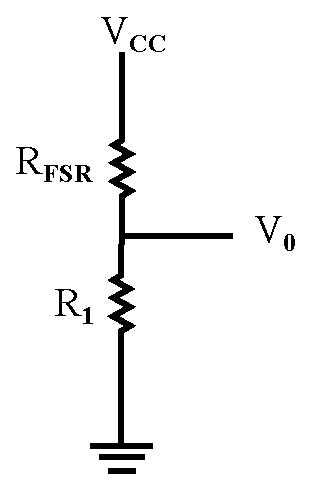
\includegraphics[width=0.3\textwidth]{./image/circuit2/circuit8_0}
\end{figure}
\end{column}

\end{columns}

\end{frame}

%------------------------------------------------
%------------------------------------------------

\begin{frame}
\frametitle{Solution(Q8(a))}
\begin{itemize} \itemsep1pt \parskip0pt \parsep0pt
  \item[$\ast$] You have to design a hammer machine(i.e. using a hammer to hit a platform to see how strong the participants are). The design goal is to generate an output voltage ($V_o$) which is proportional to the force($F$) applied on the hammer, i.e. $V_o = m \times F + C$, with $m > 0$ and $C > 0$.
  \item[$\ast$] \blue{(a) You found a force-sensitive resistor (FSR) from the catalog, which can be modeled by $R_{FSR} = 10k\Omega/F$}
\end{itemize}

\begin{columns}

\begin{column}{6.6cm}
\begin{itemize} \itemsep1pt \parskip0pt \parsep0pt
  \item[] \blue{You then design a circuit as a potential divider. Will this circuit correctly implement?}
  \item[$A:$] \red{\bf No}, because $V_o$ is not linearly proportional to $F$.
  \item[] ($V_o = V_{cc} \cdot \frac{R_1}{R_1 + R_{FSR}} = V_{cc} \cdot \frac{R_1}{R_1 + \frac{10k\Omega}{F}}$)
\end{itemize}
\end{column}


\begin{column}{6cm}
\begin{figure}[H]
  \centering
  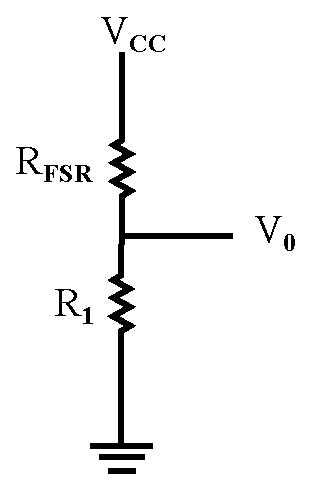
\includegraphics[width=0.3\textwidth]{./image/circuit2/circuit8_0}
\end{figure}
\end{column}

\end{columns}

\end{frame}

%------------------------------------------------
%------------------------------------------------

\begin{frame}
\frametitle{Question 8(b)}
\begin{itemize} \itemsep1pt \parskip0pt \parsep0pt
  \item[$\ast$] (b) Find the gain of the following circuit:
\end{itemize}

\begin{columns}

\begin{column}{6cm}

\end{column}


\begin{column}{6cm}
\begin{figure}[H]
  \centering
  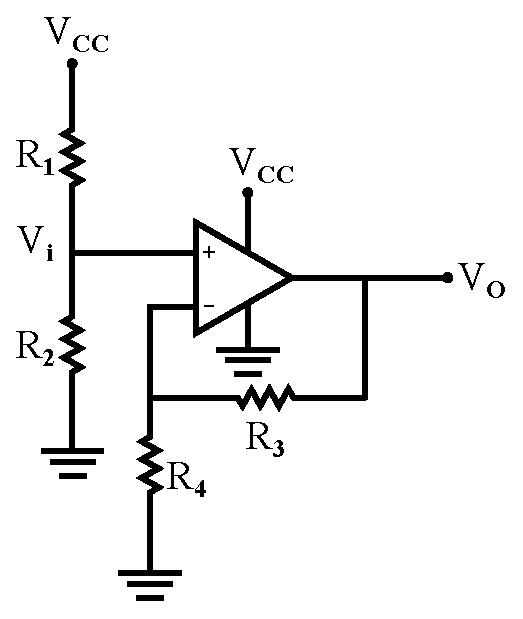
\includegraphics[width=0.6\textwidth]{./image/circuit2/circuit8_1}
\end{figure}
\end{column}

\end{columns}

\end{frame}

%------------------------------------------------
%------------------------------------------------

\begin{frame}
\frametitle{Solution(Q8(b))}
\begin{itemize} \itemsep1pt \parskip0pt \parsep0pt
  \item[$\ast$] \blue{(b) Find the gain of the following circuit:}
  \item[$\ast$] At the two op-amp inputs, $V_- = V_+ = V_i$.
  \item[$\ast$] Since $V_i$ is related to $V_o$ through the two resistors such that $V_i = V_- = \frac{R_4}{R_3 + R_4}V_o$,
  \item[] $\Rightarrow V_o = $\red{$(1 + \frac{R_3}{R_4})$}$V_i$
\end{itemize}




\begin{figure}[H]
  \centering
  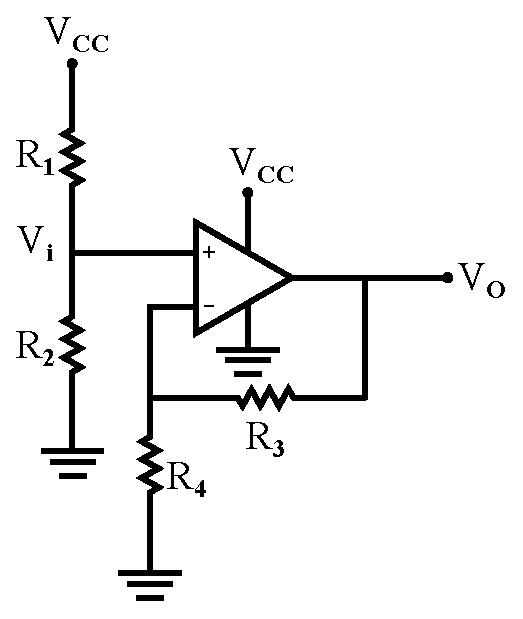
\includegraphics[width=0.3\textwidth]{./image/circuit2/circuit8_1}
\end{figure}


\end{frame}

%------------------------------------------------
%------------------------------------------------

\begin{frame}
\frametitle{Question 8(c)}
\begin{itemize} \itemsep1pt \parskip0pt \parsep0pt
  \item[$\ast$] (c) Design(by using the {\bf non-inverting} amplifier circuit) a circuit such that the output voltage($V_o$) is directly proportional to the input force($F$).
\end{itemize}

\begin{columns}

\begin{column}{6cm}

\end{column}


\begin{column}{6cm}
\begin{figure}[H]
  \centering
  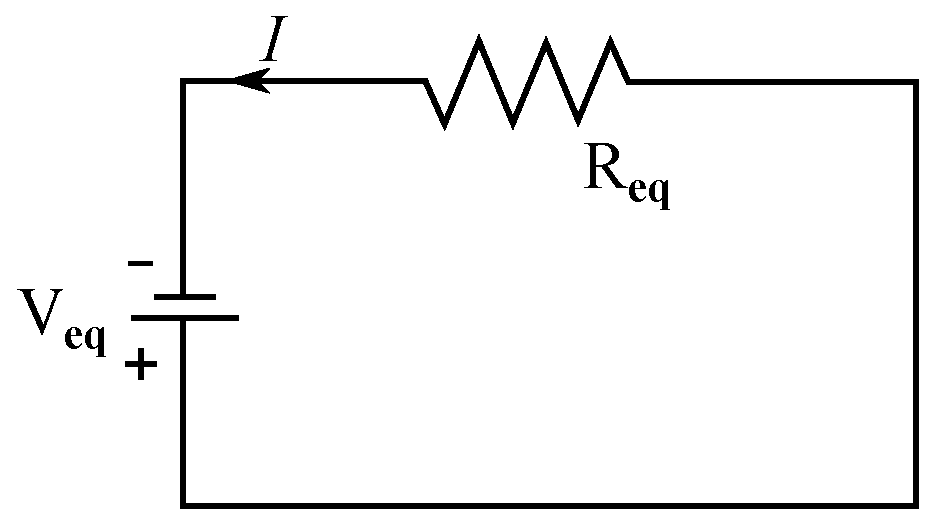
\includegraphics[width=0.6\textwidth]{./image/circuit2/circuit8_2}
\end{figure}
\end{column}

\end{columns}

\end{frame}

%------------------------------------------------
%------------------------------------------------

\begin{frame}
\frametitle{Solution(Q8(c))}
\begin{itemize} \itemsep1pt \parskip0pt \parsep0pt
  \item[$\ast$] \blue{(c) Design (by using the {\bf non-inverting} amplifier circuit) a circuit such that the output voltage ($V_o$) is directly proportional to the input force($F$).}
\end{itemize}


\begin{columns}

\begin{column}{8cm}
\begin{itemize} \itemsep1pt \parskip0pt \parsep0pt
  \item[$\ast$] Replace $R_4$ by the FSR. We then have
  \item[] $V_o = (1 + \frac{R_3F}{10000})V_i = \frac{R_3V_i}{10000}F + V_i$
  \item[] $V_o$ is a linear function of $F$
\end{itemize}
\end{column}


\begin{column}{4cm}
\begin{figure}[H]
  \centering
  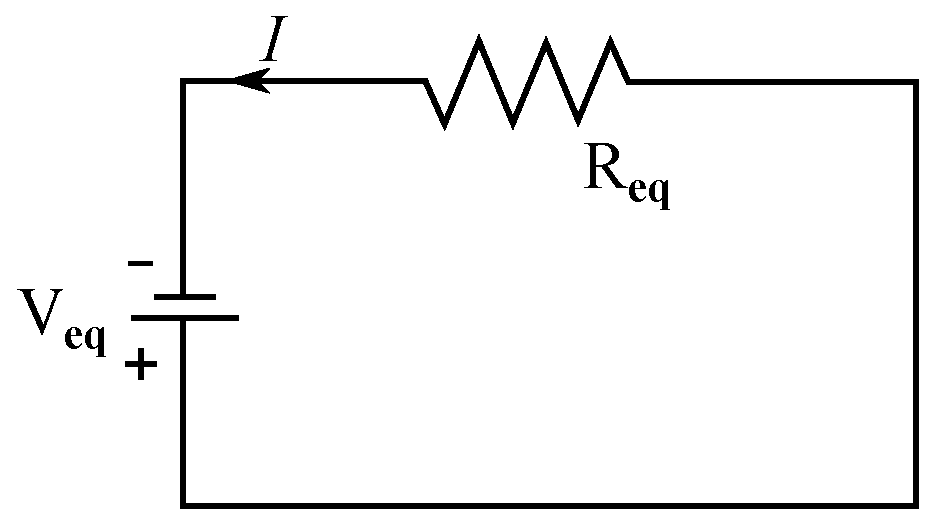
\includegraphics[width=1\textwidth]{./image/circuit2/circuit8_2}
\end{figure}
\end{column}

\end{columns}



\end{frame}

%------------------------------------------------
%------------------------------------------------

\begin{frame}
\frametitle{Question 8(d)}
\begin{itemize} \itemsep1pt \parskip0pt \parsep0pt
  \item[$\ast$] (d) The system requires that
  \begin{itemize} \itemsep1pt \parskip0pt \parsep0pt
    \item[$\ast$] when the force $F = 0N$, the output voltage $V_o = 4V$
    \item[$\ast$] when $F = 20N$, $V_o = 12V$
    \item[$\ast$] Construct the circuit designed in (c) using only {\bf one FSR}, {\bf one op-amp}, {\bf one $12V$ power supply}, and an {\bf unlimited} number of $1k\Omega$ {\bf resistors}.
  \end{itemize}
\end{itemize}
\begin{figure}[H]
  \centering
  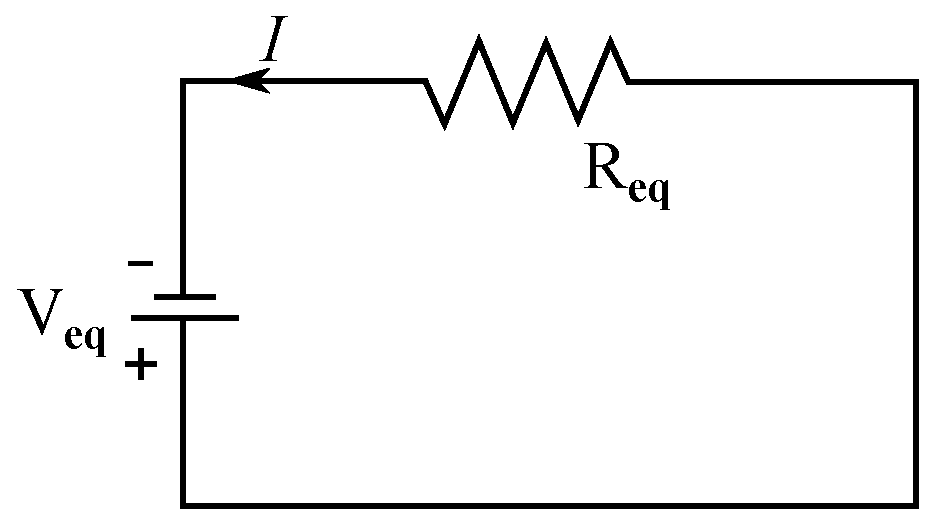
\includegraphics[width=0.3\textwidth]{./image/circuit2/circuit8_2}
\end{figure}

\end{frame}

%------------------------------------------------
%------------------------------------------------

\begin{frame}
\frametitle{Solution(Q8(d))}

\begin{columns}
\begin{column}{8cm}


\begin{itemize} \itemsep1pt \parskip0pt \parsep0pt
  \item[] \red{$V_o = (1 + \frac{R_3F}{10000})V_i = \frac{R_3V_i}{10000}F + V_i$}
  \vspace{8 mm}
  \item[] \blue{(d) The system requires that}
  \begin{itemize} \itemsep1pt \parskip0pt \parsep0pt
  \item[] \blue{when the force $F = 0N$, $V_o = 4V$}
  \item[] \blue{when $F = 20N$, $V_o = 12V$}
  \end{itemize}
\end{itemize}
\end{column}


\begin{column}{4cm}
\begin{figure}[H]
  \centering
  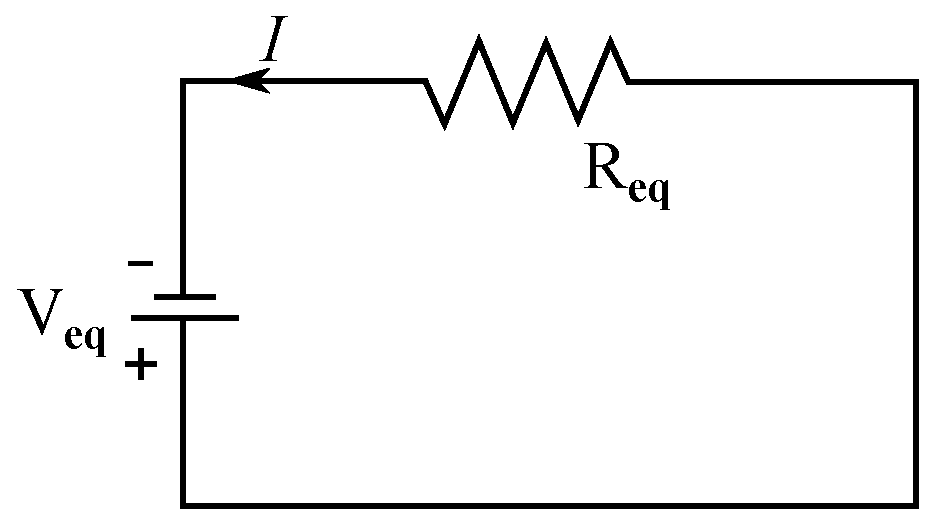
\includegraphics[width=0.8\textwidth]{./image/circuit2/circuit8_2}
\end{figure}
\end{column}
\end{columns}



\begin{itemize} \itemsep1pt \parskip0pt \parsep0pt
  \item[$\ast$] \blue{Construct the circuit designed in (c) using only one FSR, one op-amp, one 12V power supply, and 1k ohm resis.}
  \item[$\ast$] When $F = 0N$, $V_o = V_i = 4V$. We can use $R_1 = 2k\Omega$ and $R_2 = 1k\Omega$($2k\Omega$ resistors can be made by two $1k\Omega$ resistors in series). When F = 20N,
  \item[] \hspace{25 mm}\red{$12 = \frac{R_3 \times 4}{10000} \times 20 + 4 \Leftarrow R_3 = 1k\Omega$}
\end{itemize}



\end{frame}

%------------------------------------------------
%------------------------------------------------

\begin{frame}
\frametitle{Question 8(e\&f)}
\begin{itemize} \itemsep1pt \parskip0pt \parsep0pt
  \item[$\ast$] (e) Using the above circuit, what is the value of $V_o$ when someone hits the hammer too hard, generating a force of $200N$?
  \item[$\ast$] (f) Suggest modification(s) to your answer in Part (d) such that the maximum allowable force to the circuit is $60N$. You can only use the available components in Part(d), while maintaining $V_o$ to be directly proportional to $F$.
\end{itemize}

\vspace{6 cm}

\end{frame}

%------------------------------------------------
%------------------------------------------------

\begin{frame}
\frametitle{Solution(Q8(e\&f))}

\begin{columns}
\begin{column}{8cm}


\begin{itemize} \itemsep1pt \parskip0pt \parsep0pt
  \item[] \red{$V_o = (1 + \frac{R_3F}{10000})V_i = \frac{R_3V_i}{10000}F + V_i$}
  \vspace{8 mm}
  \item[] \blue{(e) Using the above circuit, what is the value of $V_o$ when someone hits the hammer too hard, generating a force of $200N$?}
  \item[$A:$] \red{\bf 12V}
  \item[] \orange{\bf Notice: the op-amp is working in the saturate state}
\end{itemize}
\end{column}


\begin{column}{4cm}
\begin{figure}[H]
  \centering
  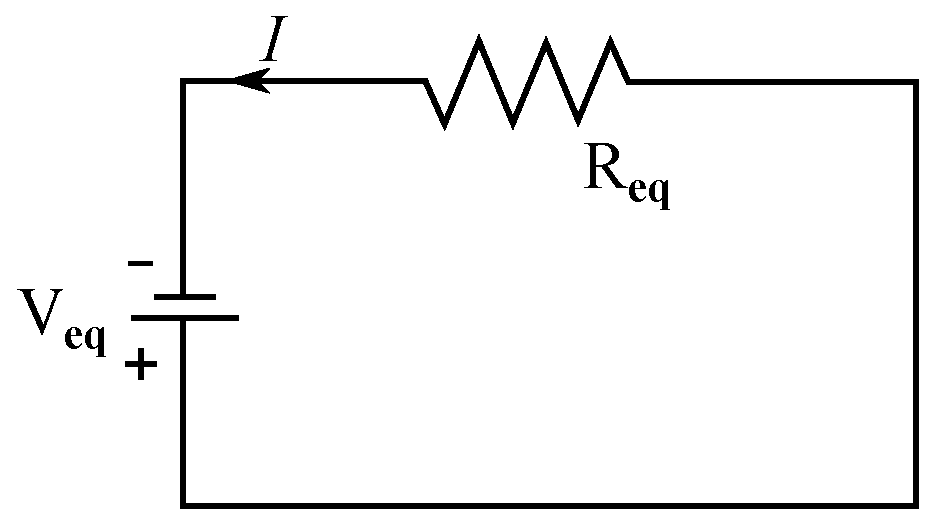
\includegraphics[width=0.8\textwidth]{./image/circuit2/circuit8_2}
\end{figure}
\end{column}
\end{columns}



\begin{itemize} \itemsep1pt \parskip0pt \parsep0pt
  \item[] \blue{(f) Suggest modification(s) such that the max allowable force to the circuit is $60N$.}
  \item[$A:$] Change $R_3$ to \red{$\frac{1}{3}k\Omega$}. This can be done by parallel composition of three $1k\Omega$ resistors.
\end{itemize}



\end{frame}

%------------------------------------------------
%------------------------------------------------

\begin{frame}
\frametitle{Appendix(Question 9)}
\begin{itemize} \itemsep1pt \parskip0pt \parsep0pt
  \item[$\ast$] Fill in the values of $R_1$ and $R_2$ required to satisfy the equations in the left column of the following table. The values must be non-negative (i.e., in the range $[0,\infty]$)
\end{itemize}

\begin{columns}
\begin{column}{6cm}

\begin{table}
\begin{center}
\def\arraystretch{1.5}

\begin{tabular}{|c|c|c|}
\hline
{} & ~~{\bf $R_1$}~~ & ~~{\bf $R_2$}~~ \\ 
\hline
$V_o = 2V_2-2V_1$ & {} & {} \\
\hline
$V_o = V_2 - V_1$ & {} & {} \\
\hline
$V_o = 4V_2-2V_1$ & {} & {} \\
\hline
\end{tabular}
\end{center}
\end{table}

\end{column}


\begin{column}{6cm}

\begin{figure}[H]
  \centering
  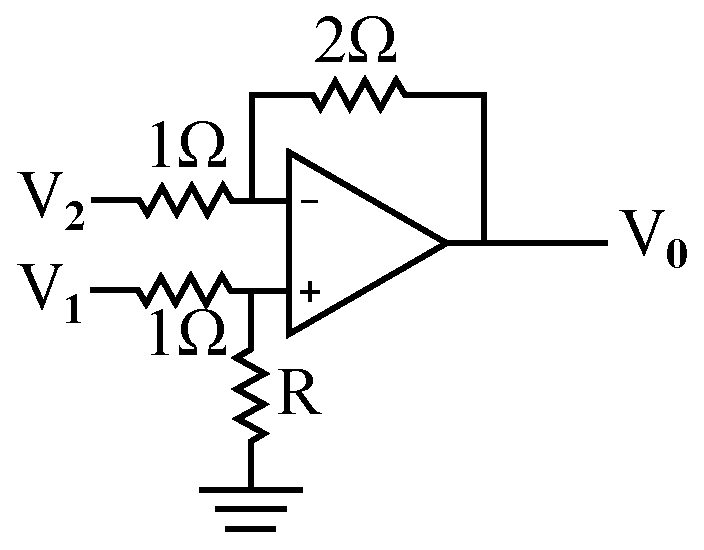
\includegraphics[width=0.8\textwidth]{./image/circuit2/circuit5_0}
\end{figure}

\end{column}
\end{columns}
\end{frame}

%------------------------------------------------
%------------------------------------------------

\begin{frame}
\frametitle{Appendix(Solution(Q9))}
\begin{itemize} \itemsep1pt \parskip0pt \parsep0pt
  \item[$\ast$] $V_+ = \frac{R_2}{10k+R_2}V_2 = V_- = \frac{R_1}{10k+R_1}V_1+\frac{10k}{10k+R_1}V_o$
  \item[$\ast$] $V_o = \frac{10k+R_1}{10k+R_2} \times \frac{R_2}{10k} \times V_2 - \frac{R_1}{10k} \times V_1$
\end{itemize}

\begin{columns}
\begin{column}{4cm}

\begin{itemize} \itemsep1pt \parskip0pt \parsep0pt
  \item[$\ast$] $3^{rd}$: Negative $R$ i.e. Impossible
\end{itemize}

\end{column}

\begin{column}{1cm}

\centerline{$\Rightarrow$}

\end{column}

\begin{column}{8cm}

\begin{table}
\begin{center}
\def\arraystretch{1.5}

\begin{tabular}{|c|c|c|}
\hline
{} & ~~{\bf $R_1$}~~ & ~~{\bf $R_2$}~~ \\ 
\hline
$V_0 = 2V_2-2V_1$ & $20k\Omega$ & $20k\Omega$ \\
\hline
$V_0 = V_2 - V_1$ & $10k\Omega$ & $10k\Omega$ \\
\hline
$V_0 = 4V_2-2V_1$ & Impossible & Impossible \\
\hline
\end{tabular}
\end{center}
\end{table}

\end{column}
\end{columns}
\end{frame}

%------------------------------------------------
%------------------------------------------------

\begin{frame}
\frametitle{Appendix(Question 10)}
\begin{itemize} \itemsep1pt \parskip0pt \parsep0pt
  \item[$\ast$] What is $V_o$?
\end{itemize}

\begin{columns}
\begin{column}{6cm}

\begin{figure}[H]
  \centering
  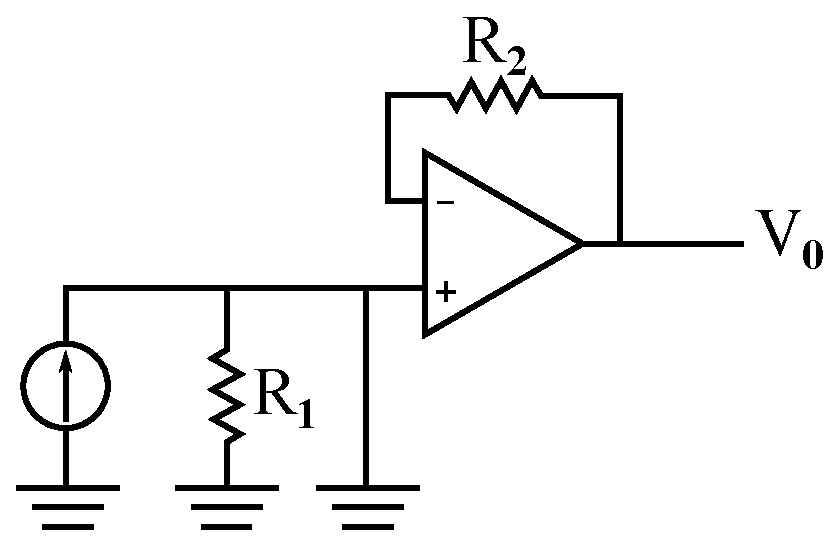
\includegraphics[width=1\textwidth]{./image/circuit2/circuit10_0}
\end{figure}

\end{column}


\begin{column}{6cm}

\begin{figure}[H]
  \centering
  \includegraphics[width=1\textwidth]{./image/circuit2/circuit10_1}
\end{figure}

\end{column}
\end{columns}
\end{frame}
%------------------------------------------------
%------------------------------------------------

\begin{frame}
\frametitle{Appendix(Solution(Q10))}
\begin{itemize} \itemsep1pt \parskip0pt \parsep0pt
  \item[$\ast$] What is $V_o$?
\end{itemize}

\begin{columns}
\begin{column}{6cm}

\begin{figure}[H]
  \centering
  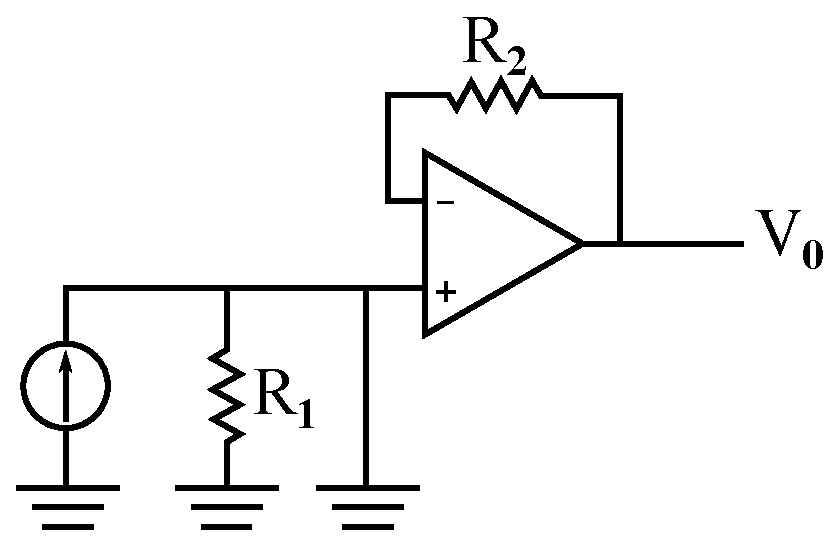
\includegraphics[width=1\textwidth]{./image/circuit2/circuit10_0}
\end{figure}
\begin{itemize} \itemsep1pt \parskip0pt \parsep0pt
  \item[] \centerline{$V_o = 0$}
\end{itemize}
\end{column}


\begin{column}{6cm}

\begin{figure}[H]
  \centering
  \includegraphics[width=1\textwidth]{./image/circuit2/circuit10_1}
\end{figure}
\begin{itemize} \itemsep1pt \parskip0pt \parsep0pt
  \item[] \centerline{$V_o = V_1 - V_2$}
\end{itemize}
\end{column}
\end{columns}
\end{frame}

%------------------------------------------------
%------------------------------------------------

\begin{frame}
\frametitle{Appendix(Question 11)}
\begin{itemize} \itemsep1pt \parskip0pt \parsep0pt
  \item[$\ast$] Students Kim, Pat, Jody, Chris, and Leon are trying to design a controller for a display of three robotic mice in the Rube Goldberg Machine, using a $10V$ power supply and three motors.
  \begin{itemize} \itemsep1pt \parskip0pt \parsep0pt
    \item[$\ast$] The first is supposed to spin as fast as possible (in one direction only), the second at half of the speed of the first, and the third at half of the speed of the second.
    \item[$\ast$] Assume the motors have a resistance of approximately \red{$5\Omega$} and that rotational speed is proportional to voltage.
  \end{itemize}
  \item[$\ast$] For each design, indicate the voltage across each of the motors.
\end{itemize}


\end{frame}

%------------------------------------------------
%------------------------------------------------

\begin{frame}
\frametitle{Appendix(Solution(Q11 -- Jody's Design))}
\begin{columns}
\begin{column}{6.5cm}
\begin{itemize} \itemsep1pt \parskip0pt \parsep0pt
  \item[] P.D. of motor 1 = $10V$
  \item[] P.D. of motor 2 = $0.05V$
  \item[] P.D. of motor 3 = $0V$
  \item[] \orange{\bf Wrong design}
\end{itemize}

\begin{itemize} \itemsep1pt \parskip0pt \parsep0pt
  \item[] \red{Eq. R.(Red): $1K + \sim 5 \rightarrow 1K$}
  \item[] \cyan{Eq. R.(Blue): $1K \parallel 1K \parallel 5 \rightarrow \sim 5$}
\end{itemize}
\end{column}


\begin{column}{5.5cm}
\begin{figure}[H]
  \centering
  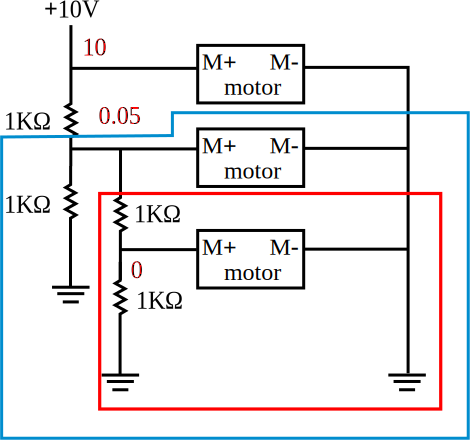
\includegraphics[width=1\textwidth]{./image/circuit2/circuit11_0}
\end{figure}
\end{column}
\end{columns}

\end{frame}

%------------------------------------------------
%------------------------------------------------

\begin{frame}
\frametitle{Appendix(Solution(Q11 -- Chris's Design))}
\begin{columns}
\begin{column}{6.5cm}
\begin{itemize} \itemsep1pt \parskip0pt \parsep0pt
  \item[] P.D. of motor 1 = $10V$
  \item[] P.D. of motor 2 = $0.45V$
  \item[] P.D. of motor 3 = $0V$
  \item[] \orange{\bf Wrong design}
\end{itemize}

\begin{itemize} \itemsep1pt \parskip0pt \parsep0pt
  \item[] \red{Eq. R.(Red): $100K + \sim 5 \rightarrow 100K$}
  \item[] \cyan{Eq. R.: $100 \parallel 100K \parallel 5 \rightarrow \sim 5$}
\end{itemize}
\end{column}


\begin{column}{5.5cm}
\begin{figure}[H]
  \centering
  \includegraphics[width=1\textwidth]{./image/circuit2/circuit11_1}
\end{figure}
\end{column}
\end{columns}

\end{frame}

%------------------------------------------------
%------------------------------------------------

\begin{frame}
\frametitle{Appendix(Solution(Q11 -- Pat's Design))}
\begin{columns}
\begin{column}{5.5cm}
\begin{itemize} \itemsep1pt \parskip0pt \parsep0pt
  \item[] P.D. of motor 1 = $10V$
  \item[] P.D. of motor 2 = $4V$
  \item[] P.D. of motor 3 = $2V$
  \item[] \orange{\bf Wrong design}
\end{itemize}

\begin{itemize} \itemsep1pt \parskip0pt \parsep0pt
  \item[] \magenta{Eq. R.: $1K \parallel 2K = \frac{2}{3}K$}
\end{itemize}
\end{column}


\begin{column}{6.5cm}
\begin{figure}[H]
  \centering
  \includegraphics[width=1\textwidth]{./image/circuit2/circuit11_2}
\end{figure}
\end{column}
\end{columns}

\end{frame}

%------------------------------------------------
%------------------------------------------------

\begin{frame}
\frametitle{Appendix(Solution(Q11 -- Kim's Design))}
\begin{columns}
\begin{column}{5.5cm}
\begin{itemize} \itemsep1pt \parskip0pt \parsep0pt
  \item[] P.D. of motor 1 = $10V$
  \item[] P.D. of motor 2 = $5V$
  \item[] P.D. of motor 3 = $2.5V$
  \item[] \green{\bf Correct design}
\end{itemize}

\begin{itemize} \itemsep1pt \parskip0pt \parsep0pt
  \item[] \magenta{Eq. R.: $100 \parallel 200K = \sim 100$}
\end{itemize}
\end{column}


\begin{column}{6.5cm}
\begin{figure}[H]
  \centering
  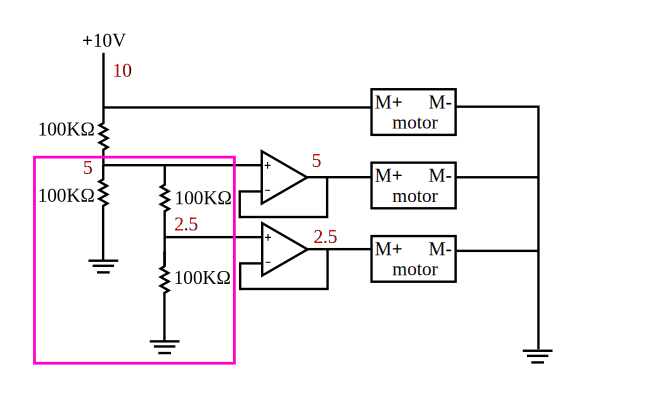
\includegraphics[width=1\textwidth]{./image/circuit2/circuit11_3}
\end{figure}
\end{column}
\end{columns}

\end{frame}

%------------------------------------------------
%------------------------------------------------

\begin{frame}
\frametitle{Appendix(Solution(Q11 -- Leon's Design))}
\begin{columns}
\begin{column}{5cm}
\begin{itemize} \itemsep1pt \parskip0pt \parsep0pt
  \item[] P.D. of motor 1 = $10V$
  \item[] P.D. of motor 2 = $5V$
  \item[] P.D. of motor 3 = $2.5V$
  \item[] \green{\bf Correct design}
\end{itemize}
\end{column}



\begin{column}{7cm}
\begin{figure}[H]
  \centering
  \includegraphics[width=1\textwidth]{./image/circuit2/circuit11_4}
\end{figure}
\end{column}
\end{columns}

\end{frame}

%------------------------------------------------
%------------------------------------------------
\begin{frame}
\frametitle{Summary}

\begin{itemize} \itemsep1pt \parskip0pt \parsep0pt
	\item[] Operational Amplifiers
  \begin{itemize} \itemsep1pt \parskip0pt \parsep0pt
    \item[$\bullet$] Ideal Op-amp Model(Properties)
    \begin{itemize}
      \item[$(1)$] $I_p = I_n = 0$
      \item[$(2)$] $R_i \rightarrow \infty$
      \item[$(3)$] $R_o = 0$
      \item[$(4)$] $A \rightarrow \infty$
    \end{itemize}
    \item[$\bullet$] Ideal op-amp in a negative feedback configuration(conditions)
    \begin{itemize}
      \item[$(1)$] $I_p = I_n = 0$: input current constraint
      \item[$(2)$] $V_n = V_p$: \hspace{4 mm}input voltage constraint
    \end{itemize}
  \end{itemize}
\end{itemize}

\end{frame}

%------------------------------------------------














% %------------------------------------------------

\begin{frame}
\Huge{\centerline{The End}}
\end{frame}

%----------------------------------------------------------------------------------------

\end{document}